\documentclass{article}
\author{Max Springenberg, 177792}
\title{
    RvS UB02\\
    Gruppe 4
}
\date{}
\usepackage{amsmath}
\usepackage{amssymb}
\usepackage{stmaryrd}
\usepackage{graphicx}
\setcounter{section}{2}
% \Theta \Omega \omega
\newcommand{\tab}{\null \qquad}
\newcommand{\lA}{$\leftarrow$}
\newcommand{\ue}{$\infty$}
\newcommand{\gap}{\\ \ \\}
\newcommand{\headline}[1]{\textbf{\textit{#1}}\\}

\begin{document}
\maketitle
\newpage

\subsection{Multiplexing}

\subsubsection{Skizzieren sie Frequenzmultiplexing (FDM)}
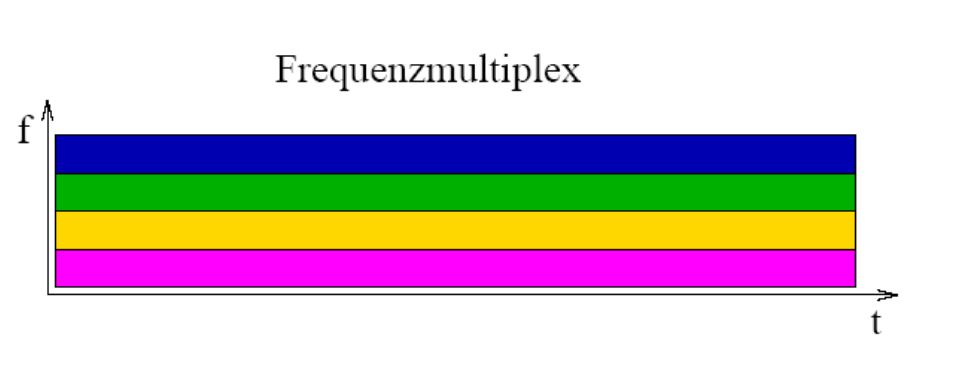
\includegraphics[width=1\textwidth]{FreqMult.png}

\subsubsection{
    Die Technik des Frequenzmultiplexing (FDM) erlaubt es in der 
    Theorie, uneingeschränkt viele Nutzer zu einem Zeitpunkt 
    übertragen zu lassen. Warum ist dies praktisch nicht umsetzbar?
}
Die Bandbreite wird beim multiplexen aufgeteilt. 
Sei $B$ die Bandbreite und $n$ die Anzahl von Usern, denen Frequenzen
zugeteilt werden. Die relative bandbreite $\delta_n(B) = \frac{B}{n}$
ergibt sich mit $n \to \infty$ zu
$$
\lim_{n \to \infty} \delta_n(B) = 0
$$\\
Damit ist uneingeschraenkte Nutzung nicht moeglich.\\

\subsubsection{Skizzieren Sie Zeitmultiplexing (TDM)}
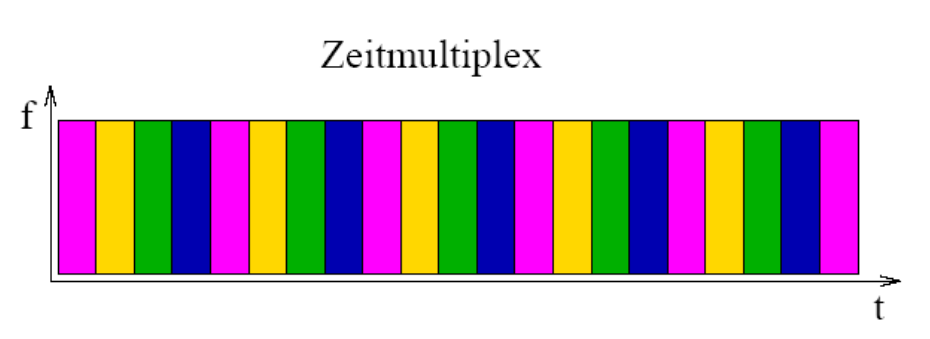
\includegraphics[width=1\textwidth]{TimeMult.png}

\subsubsection{
    Die Technik des Zeitmultiplexing (TDM) erlaubt es in der Theorie
    uneingeschränkt viele Nutzer nacheinander übertragen zu lassen. 
    Zu welchem Problem würde die Größenordnung der Nutzer bei 
    dieser Technik führen?
}
Die Bandbreite wird beim multiplexen aufgeteilt. 
Sei $n$ die Anzahl von Usern, denen Timeslots zugeteilt werden. 
Der Faktor für die Wartezeit $\delta_t(n, t) = n * t$
ergibt sich mit $n \to \infty$ zu
$$
\lim_{n \to \infty} \delta_n(n, t) = \infty
$$\\
Damit ist uneingeschraenkte Nutzung auch hier nicht moeglich.\\

\subsection{Paket- und leitungsvermittelnde Netze}

\subsubsection{
    Vergleichen Sie paketvermittelnde und leitungsvermittelnde Netze.
    Welche Vor- und Nachteile bieten beide Strategien für 
    verschiedene Applikationen?
}
\headline{Paketvermittelnd}
\begin{tabular}{l|l}
    PRO & CON\\
    \hline
    Hohe Kapazitaet&
        keine garantierte Bandbreite\\
\end{tabular}\\
\gap
\headline{Leitungsvermittelnd}
\begin{tabular}{l|l}
    PRO & CON\\
    \hline
    Volle Bandbreite&
        Geringere Kapazitaet\\
    Keine Nutzungskonkurrenz&
        \\
\end{tabular}\\

\subsubsection{
    Bei den paketvermittelnden Netzen werden verbindungslose und 
    verbindungsorientierte Dienste angeboten.
}
\headline{Wo liegen die Unterschiede?}
\begin{tabular}{l|c|c}
        &Verbindungsorientiert&Verbindungslos\\
    Handshake&
        Ja&Nein\\
    \hline
    Protokoll&
        TCP&UDP\\
    Zuverlaessiger Datentransfer&
        Ja&Nein\\
    Flusskontrolle&
        Ja&Nein\\
    Ueberlastkontrolle&
        Ja&Nein\\
    \hline
    Paketverluste&
        Nein&Moeglich\\
\end{tabular}\\
\gap
\headline{Gibt es diese Unterscheidung auch bei leitungsvermittelnden Netzen?} 
Nein, das Problem behandelt eine konkurrente Paketuebertragung.\\

\subsection{TCP/IP}
\subsubsection{
    Geben Sie fuer den TCP/IP-Protokollstack beispielhaft die 
    Protokolle der einzelnen Schichten, sowie die Dienste,
    welche diese zur Verfügung stellen, an.
}
%\includegraphics[width=1\textwidth]{TCP_IP_stack.png}
\begin{tabular}{l|l|l}
    Schicht & Protokolle & Dienste\\
\end{tabular}
\subsection{ISO/ OSI-Basisfrequenzmodell}
\end{document}
